% Appendix companion for the revised decomposition section.

\section{Appendix to Section~\ref{sec:decomposition}: Technical Details and Additional Diagnostics}
\label{app:decomposition}

This appendix collects the technical pieces that support the main decomposition but are not needed to follow the paper's central argument. The main text uses aggregate count accounting as the identification anchor and then uses the cohort framework to allocate effects across places, ages, and regimes. The appendix documents the exact operator, implementation rules, and supplementary diagnostics that show where the cohort framework is most credible.

\subsection{Exact cohort operator and education accounting}
\label{app:decomp_operator}

Let $N_{m,t,c,e}$ be the count of registered voters in municipality $m$, election year $t$, age cohort $c$, and education group $e \in \{L,H\}$. Denote total cohort size by $N_{m,t,c} = \sum_{e} N_{m,t,c,e}$. Let $A_{c'c}$ be the mechanical-aging matrix, where $A_{c'c}$ is the share of voters in source cohort $c'$ at $t$ who age into target cohort $c$ at $t+2$. The matrix has at most two nonzero entries per row for all nonabsorbing bins, reflecting the fact that a two-year election cycle can leave part of a source cohort in place and move the remainder into the next bin. The exact entries follow the TSE age bins: single-year bins for ages 16--20, a four-year bin for ages 21--24, five-year bins thereafter, and an absorbing 100+ bin.

Given pre-treatment survival rates $\hat\sigma_{m,c'}$, the no-BVR counterfactual for total cohort size is
\begin{equation}
\widehat N^{0}_{m,t+2,c}
=
\sum_{c'} A_{c'c}\hat\sigma_{m,c'}N_{m,t,c'} + I_{m,t+2,c},
\label{eq:app_decomp_total_counterfactual}
\end{equation}
where $I_{m,t+2,c}$ captures new registration into the youngest bins. This formulation makes explicit that a target cohort at $t+2$ can receive mass from more than one source cohort at $t$.

For the education split, let $P^{0}_{m,c',e \rightarrow e'}$ denote the pre-treatment transition probability from education group $e$ in source cohort $c'$ at $t$ to education group $e'$ at $t+2$ absent BVR. The corresponding no-BVR cell counts are
\begin{equation}
\widehat N^{0}_{m,t+2,c,e'}
=
\sum_{c',e} A_{c'c}\hat\sigma_{m,c'}N_{m,t,c',e}P^{0}_{m,c',e \rightarrow e'} + I_{m,t+2,c,e'},
\label{eq:app_decomp_cell_counterfactual}
\end{equation}
where $I_{m,t+2,c,e'}$ allows inflows into the youngest bins by education category.

For ages 35 and older, the benchmark implementation sets the natural education-progression probability from low to high education to zero over a two-year cycle. For ages 25--34, that transition is allowed but expected to be small. For ages 16--24, it is estimated from pre-treatment transitions and the resulting record-updating estimates are treated as auxiliary rather than central.

Cohort-level exit is
\begin{equation}
E_{m,t+2,c}
=
\max\left\{0,\widehat N^{0}_{m,t+2,c} - N_{m,t+2,c}\right\}.
\label{eq:app_decomp_exit}
\end{equation}
Under Scenario B, all within-cohort exit is allocated to the low-education group. Under Scenario C, exit is allocated proportionally to the no-BVR education composition within the cohort. In both cases, record updating is the residual movement from low to high education required to reconcile observed and predicted cell counts after the exit allocation is fixed. Finally, record updating in any cell is capped by observed biometric uptake:
\begin{equation}
R_{m,t+2,c}
\leq
b_{m,t+2,c}N_{m,t+2,c},
\label{eq:app_decomp_bcap}
\end{equation}
where $b_{m,t+2,c}$ is the share of the cohort with completed biometrics. This cap is usually slack in strict municipalities and informative in hybrid municipalities.

\subsection{Implementation rules and interpretation}
\label{app:decomp_methods}
\label{app:decomp_implementation}

\paragraph{Survival-rate estimation.}
The preferred estimate uses municipality-specific pre-treatment transitions when the source cohort is large enough. When the source cell is too small, the algorithm falls back to the state-level estimate for the same cohort; if that is unavailable, it uses the national cohort mean from untreated observations. If the final code uses thresholds different from the ones below, replace them before integrating the section. In the current implementation, municipality-specific survival is used when the source cell contains at least 100 voters in the single-year young bins and at least 200 voters in the multi-year bins.

\paragraph{Interpretation of exit.}
The exit component is best read as BVR-attributable loss relative to the municipality's own pre-treatment cohort dynamics. Because abnormal post-adoption out-migration and administrative cancellation are not separately observed, the municipality-level exit estimate is an upper bound on true BVR-induced removal whenever post-adoption migration deviates from the pre-treatment baseline.

\paragraph{Interpretation of record updating.}
The cleanest record-updating estimates come from working-age cohorts that are old enough for natural schooling progression to be limited but not so old that survival-rate noise dominates. For that reason, the main text emphasizes the 25--44 and 35--64 patterns and treats the youngest and oldest bins as supporting rather than central evidence.

\paragraph{How to read the regime figure.}
The stacked regime figure is a summary of the share of the baseline electorate administratively affected by the reform through either removal or record updating. It is not a decomposition of net registry contraction, because record updating changes measured composition without shrinking the total count.

% Supplementary tables for the revised decomposition section.

\subsection{Supplementary tables}
\label{app:decomp_tables}

\begin{table}[!htbp]
\centering
\caption{Raw-count version of the cohort-based allocation by first-treatment regime}
\label{tab:decomp_counts}
\label{tab:decomp_aggregate_counts_appendix}
\begin{tabular}{lcccc}
\toprule
First regime & Municipalities & Exit count & Re-labeling (B) & Re-labeling (C) \\
\midrule
Strict & 2{,}475 & 6{,}210{,}453 & 3{,}607{,}795 & 4{,}958{,}520 \\
Hybrid & 1{,}846 & 1{,}561{,}570 & 550{,}381 & 719{,}475 \\
All treated & 4{,}321 & 7{,}772{,}023 & 4{,}158{,}176 & 5{,}677{,}995 \\
\bottomrule
\end{tabular}

\vspace{0.75em}
\begin{minipage}{\textwidth}
{\footnotesize \textbf{Note:} This is the raw-count counterpart to Table~\ref{tab:decomp_aggregate}. Keeping counts in the appendix avoids mixing levels and rates in the main text while preserving the quantities needed for calibration or back-of-the-envelope comparisons. \par}
\end{minipage}
\end{table}

\begin{table}[!htbp]
\centering
\caption{Working-age restrictions for the cohort-based allocation}
\label{tab:decomp_workingage}
\begin{tabular}{lccc}
\toprule
Sample & Exit (upper bound) & Re-labeling (B) & Re-labeling (C) \\
\midrule
All ages & 8.35\% & 4.47\% & 6.10\% \\
Ages 25--64 & \textit{[fill from code]} & \textit{[fill from code]} & \textit{[fill from code]} \\
Ages 35--64 & \textit{[fill from code]} & \textit{[fill from code]} & \textit{[fill from code]} \\
\bottomrule
\end{tabular}

\vspace{0.75em}
\begin{minipage}{\textwidth}
{\footnotesize \textbf{Note:} Rates should be expressed as percentages of the restricted sample's 2008 baseline electorate. This table is the most useful robustness check for the cohort framework because it shows whether the aggregate allocation changes materially once the noisiest age bins (16--24 and 65+) are removed. If the working-age estimates are close to the all-age estimates, say so directly in the text. \par}
\end{minipage}
\end{table}

\begin{table}[!htbp]
\centering
\caption{Pre-treatment backtest of the cohort algorithm}
\label{tab:decomp_placebo}
\begin{tabular}{p{0.30\textwidth}ccc}
\toprule
Untreated cycle used as pseudo-treatment & Pseudo-exit & Pseudo-relabel B & Pseudo-relabel C \\
\midrule
2008$\rightarrow$2010 & \textit{[fill from code]} & \textit{[fill from code]} & \textit{[fill from code]} \\
2010$\rightarrow$2012 & \textit{[fill from code]} & \textit{[fill from code]} & \textit{[fill from code]} \\
Pooled untreated benchmark & \textit{[fill from code]} & \textit{[fill from code]} & \textit{[fill from code]} \\
\bottomrule
\end{tabular}

\vspace{0.75em}
\begin{minipage}{\textwidth}
{\footnotesize \textbf{Note:} Restrict each row to municipalities untreated at both dates and run the same cohort algorithm used in the main decomposition. The target is not exact zeros in every cell but small pseudo-effects relative to the post-adoption magnitudes. This is the most direct diagnostic of whether the framework is spuriously generating exit or record updating absent BVR. \par}
\end{minipage}
\end{table}

\begin{table}[!htbp]
\centering
\caption{Implementation diagnostics for the cohort framework}
\label{tab:decomp_diagnostics}
\begin{tabular}{lc}
\toprule
Diagnostic & Value \\
\midrule
Treated municipalities used in the allocation & 4{,}321 \\
Electorate-weighted share of cells using municipality-specific survival & \textit{[fill from code]} \\
Electorate-weighted share of cells using state-level fallback & \textit{[fill from code]} \\
Electorate-weighted share of cells using national fallback & \textit{[fill from code]} \\
Electorate-weighted share of cells where the biometric-uptake cap binds & \textit{[fill from code]} \\
Electorate-weighted share of cells where the non-negativity floor binds & \textit{[fill from code]} \\
Bootstrap SE for aggregate exit & \textit{[fill from code]} \\
Bootstrap SE for aggregate re-labeling (B) & \textit{[fill from code]} \\
Bootstrap SE for aggregate re-labeling (C) & \textit{[fill from code]} \\
\bottomrule
\end{tabular}

\vspace{0.75em}
\begin{minipage}{\textwidth}
{\footnotesize \textbf{Note:} This table makes the implementation transparent. If the bootstrap is not yet available, drop those rows rather than reporting conventional standard errors that ignore first-stage uncertainty. The share of cells where the uptake cap or non-negativity floor binds is particularly informative about where the framework is doing mechanical cleanup rather than delivering clean signal. \par}
\end{minipage}
\end{table}

% Supplementary figures for the revised decomposition section.

\subsection{Additional figures}
\label{app:decomp_figures}
\label{ssec:decomposition_figures}

\begin{figure}[!htbp]
\centering
\IfFileExists{../resources/decomposition/figures/figure_02_binned_scatter_exit_lowed_notitle.pdf}{%
  
\includegraphics[width=0.72\textwidth]{../resources/decomposition/figures/figure_02_binned_scatter_exit_lowed_notitle.pdf}%
}{%
  \fbox{\parbox[c][2in][c]{0.72\textwidth}{\centering Placeholder for municipality-level binned scatter.}}%
}
\caption{Municipality-level exit rate and baseline low-education share}
\label{fig:decomp_scatter_muni}
\label{fig:decomp_scatter_muni_app}

\vspace{0.75em}
\begin{minipage}{\textwidth}
{\footnotesize \textbf{Note:} This figure is a descriptive complement to the main allocation results. Because the dependent variable is itself generated by the cohort framework, the figure should be read as supportive heterogeneity rather than independent identification. \par}
\end{minipage}
\end{figure}

\begin{figure}[!htbp]
\centering
\IfFileExists{../resources/decomposition/figures/figure_03_state_scatter_exit_lowed_notitle.pdf}{%
  
\includegraphics[width=0.72\textwidth]{../resources/decomposition/figures/figure_03_state_scatter_exit_lowed_notitle.pdf}%
}{%
  \fbox{\parbox[c][2in][c]{0.72\textwidth}{\centering Placeholder for state-level scatter.}}%
}
\caption{State-level exit rate and baseline low-education share}
\label{fig:decomp_scatter_state}
\label{fig:decomp_scatter_state_app}

\vspace{0.75em}
\begin{minipage}{\textwidth}
{\footnotesize \textbf{Note:} State aggregation is useful for visual context but too coarse for identification. If retained, the text should emphasize the descriptive regional pattern rather than treat this figure as a test. \par}
\end{minipage}
\end{figure}

\begin{figure}[!htbp]
\centering
\IfFileExists{../resources/decomposition/figures/figure_04_interaction_coefficients_notitle.pdf}{%
  
\includegraphics[width=0.72\textwidth]{../resources/decomposition/figures/figure_04_interaction_coefficients_notitle.pdf}%
}{%
  \fbox{\parbox[c][2in][c]{0.72\textwidth}{\centering Placeholder for interaction coefficient plot.}}%
}
\caption{Supplementary interaction coefficients}
\label{fig:decomp_coefficients}
\label{fig:decomp_coefficients_app}

\vspace{0.75em}
\begin{minipage}{\textwidth}
{\footnotesize \textbf{Note:} This figure should remain in the appendix unless the full pipeline is bootstrapped. Otherwise the reported uncertainty conditions on a generated dependent variable and does not capture first-stage uncertainty from the cohort allocation itself. \par}
\end{minipage}
\end{figure}

\begin{figure}[!htbp]
\centering
\IfFileExists{../resources/decomposition/figures/figure_05_share_by_age_band_notitle.pdf}{%
  
\includegraphics[width=0.72\textwidth]{../resources/decomposition/figures/figure_05_share_by_age_band_notitle.pdf}%
}{%
  \fbox{\parbox[c][2in][c]{0.72\textwidth}{\centering Placeholder for age-profile figure.}}%
}
\caption{Full age profile of exit and record updating}
\label{fig:decomp_age_share}
\label{fig:decomp_age_share_app}

\vspace{0.75em}
\begin{minipage}{\textwidth}
{\footnotesize \textbf{Note:} The main text should draw attention to the working-age concentration of re-labeling rather than to the noisy oldest bins. If a redesigned main-text age figure is later added, it should focus on ages 25--64 or 35--64 and relegate the full profile to this appendix. \par}
\end{minipage}
\end{figure}

\begin{figure}[p]
    \caption{BJS imputation decomposition event studies over the 2006 baseline}
    \label{fig:appendix-decomp-event-components}
    \label{fig:appendix-decomp-event-combined}
    \centering
    \begin{subfigure}[b]{0.49\textwidth}
        \centering
        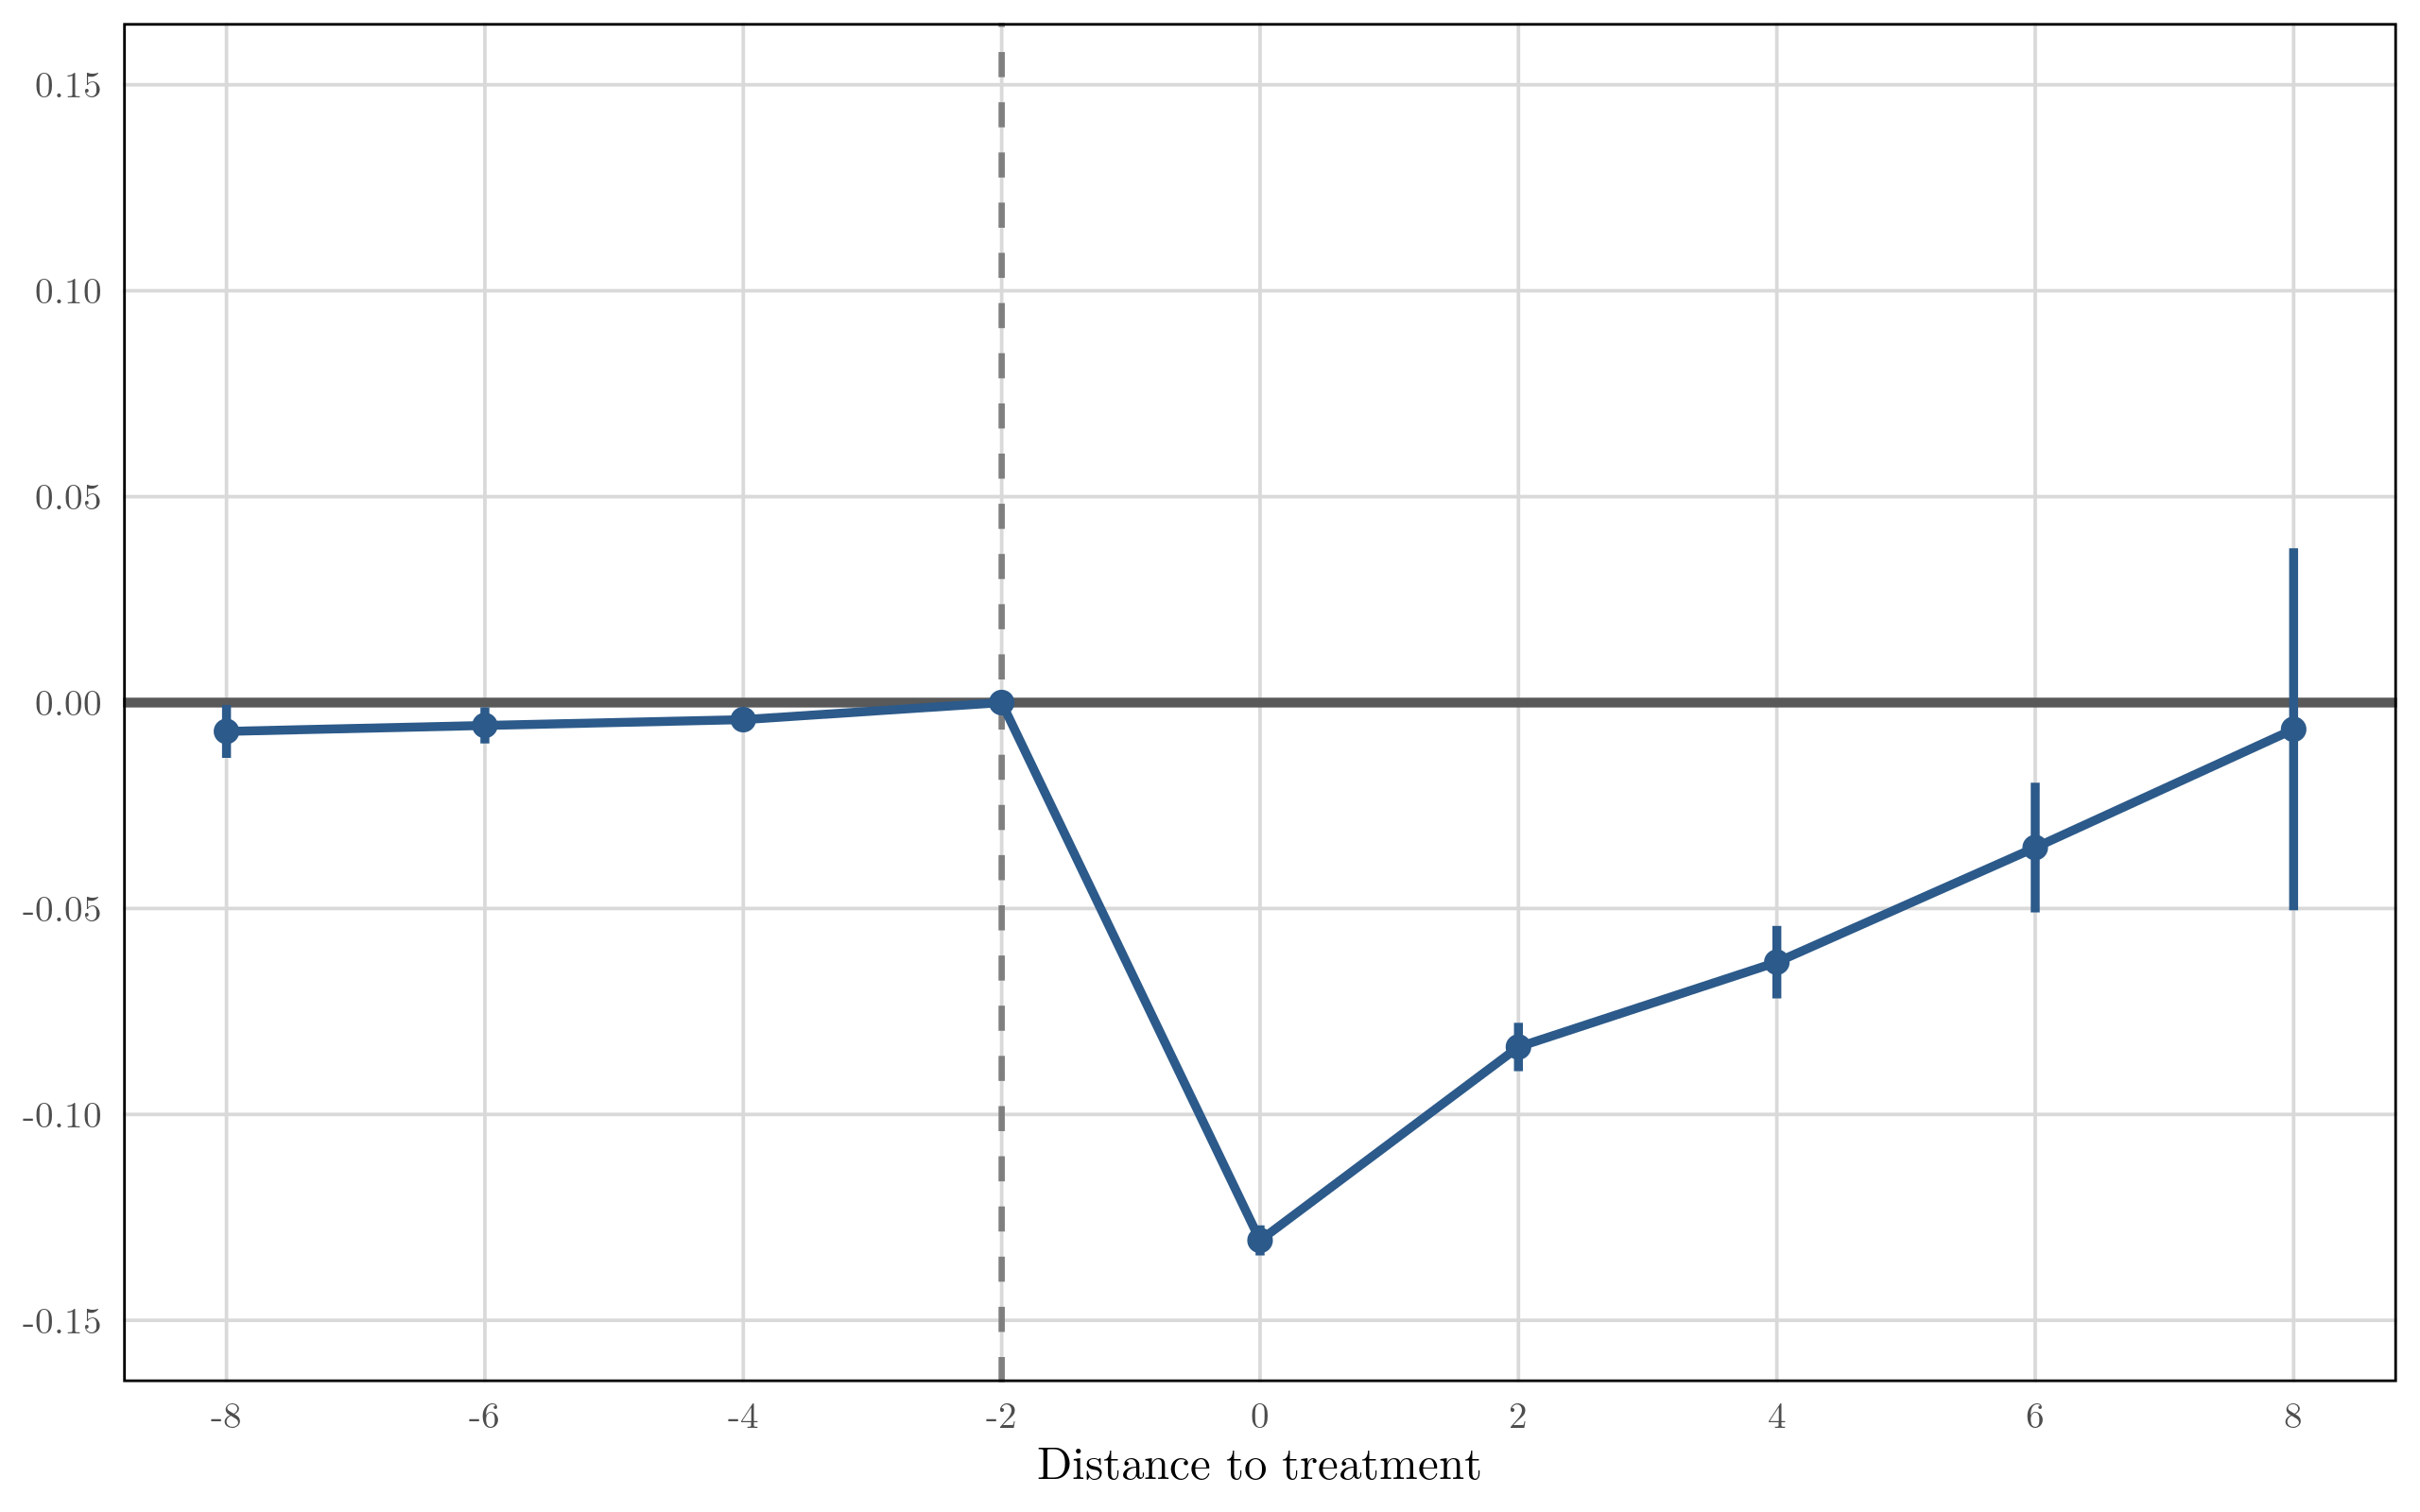
\includegraphics[width=\textwidth]{../resources/regressions/decomposition/num_voters_over_2006/strict_bvr/callaway_santanna/event_study_plot.png}
        \caption{Total electorate over 2006 total}
        \label{fig:appendix-decomp-event-total}
    \end{subfigure}
    \hfill
    \begin{subfigure}[b]{0.49\textwidth}
        \centering
        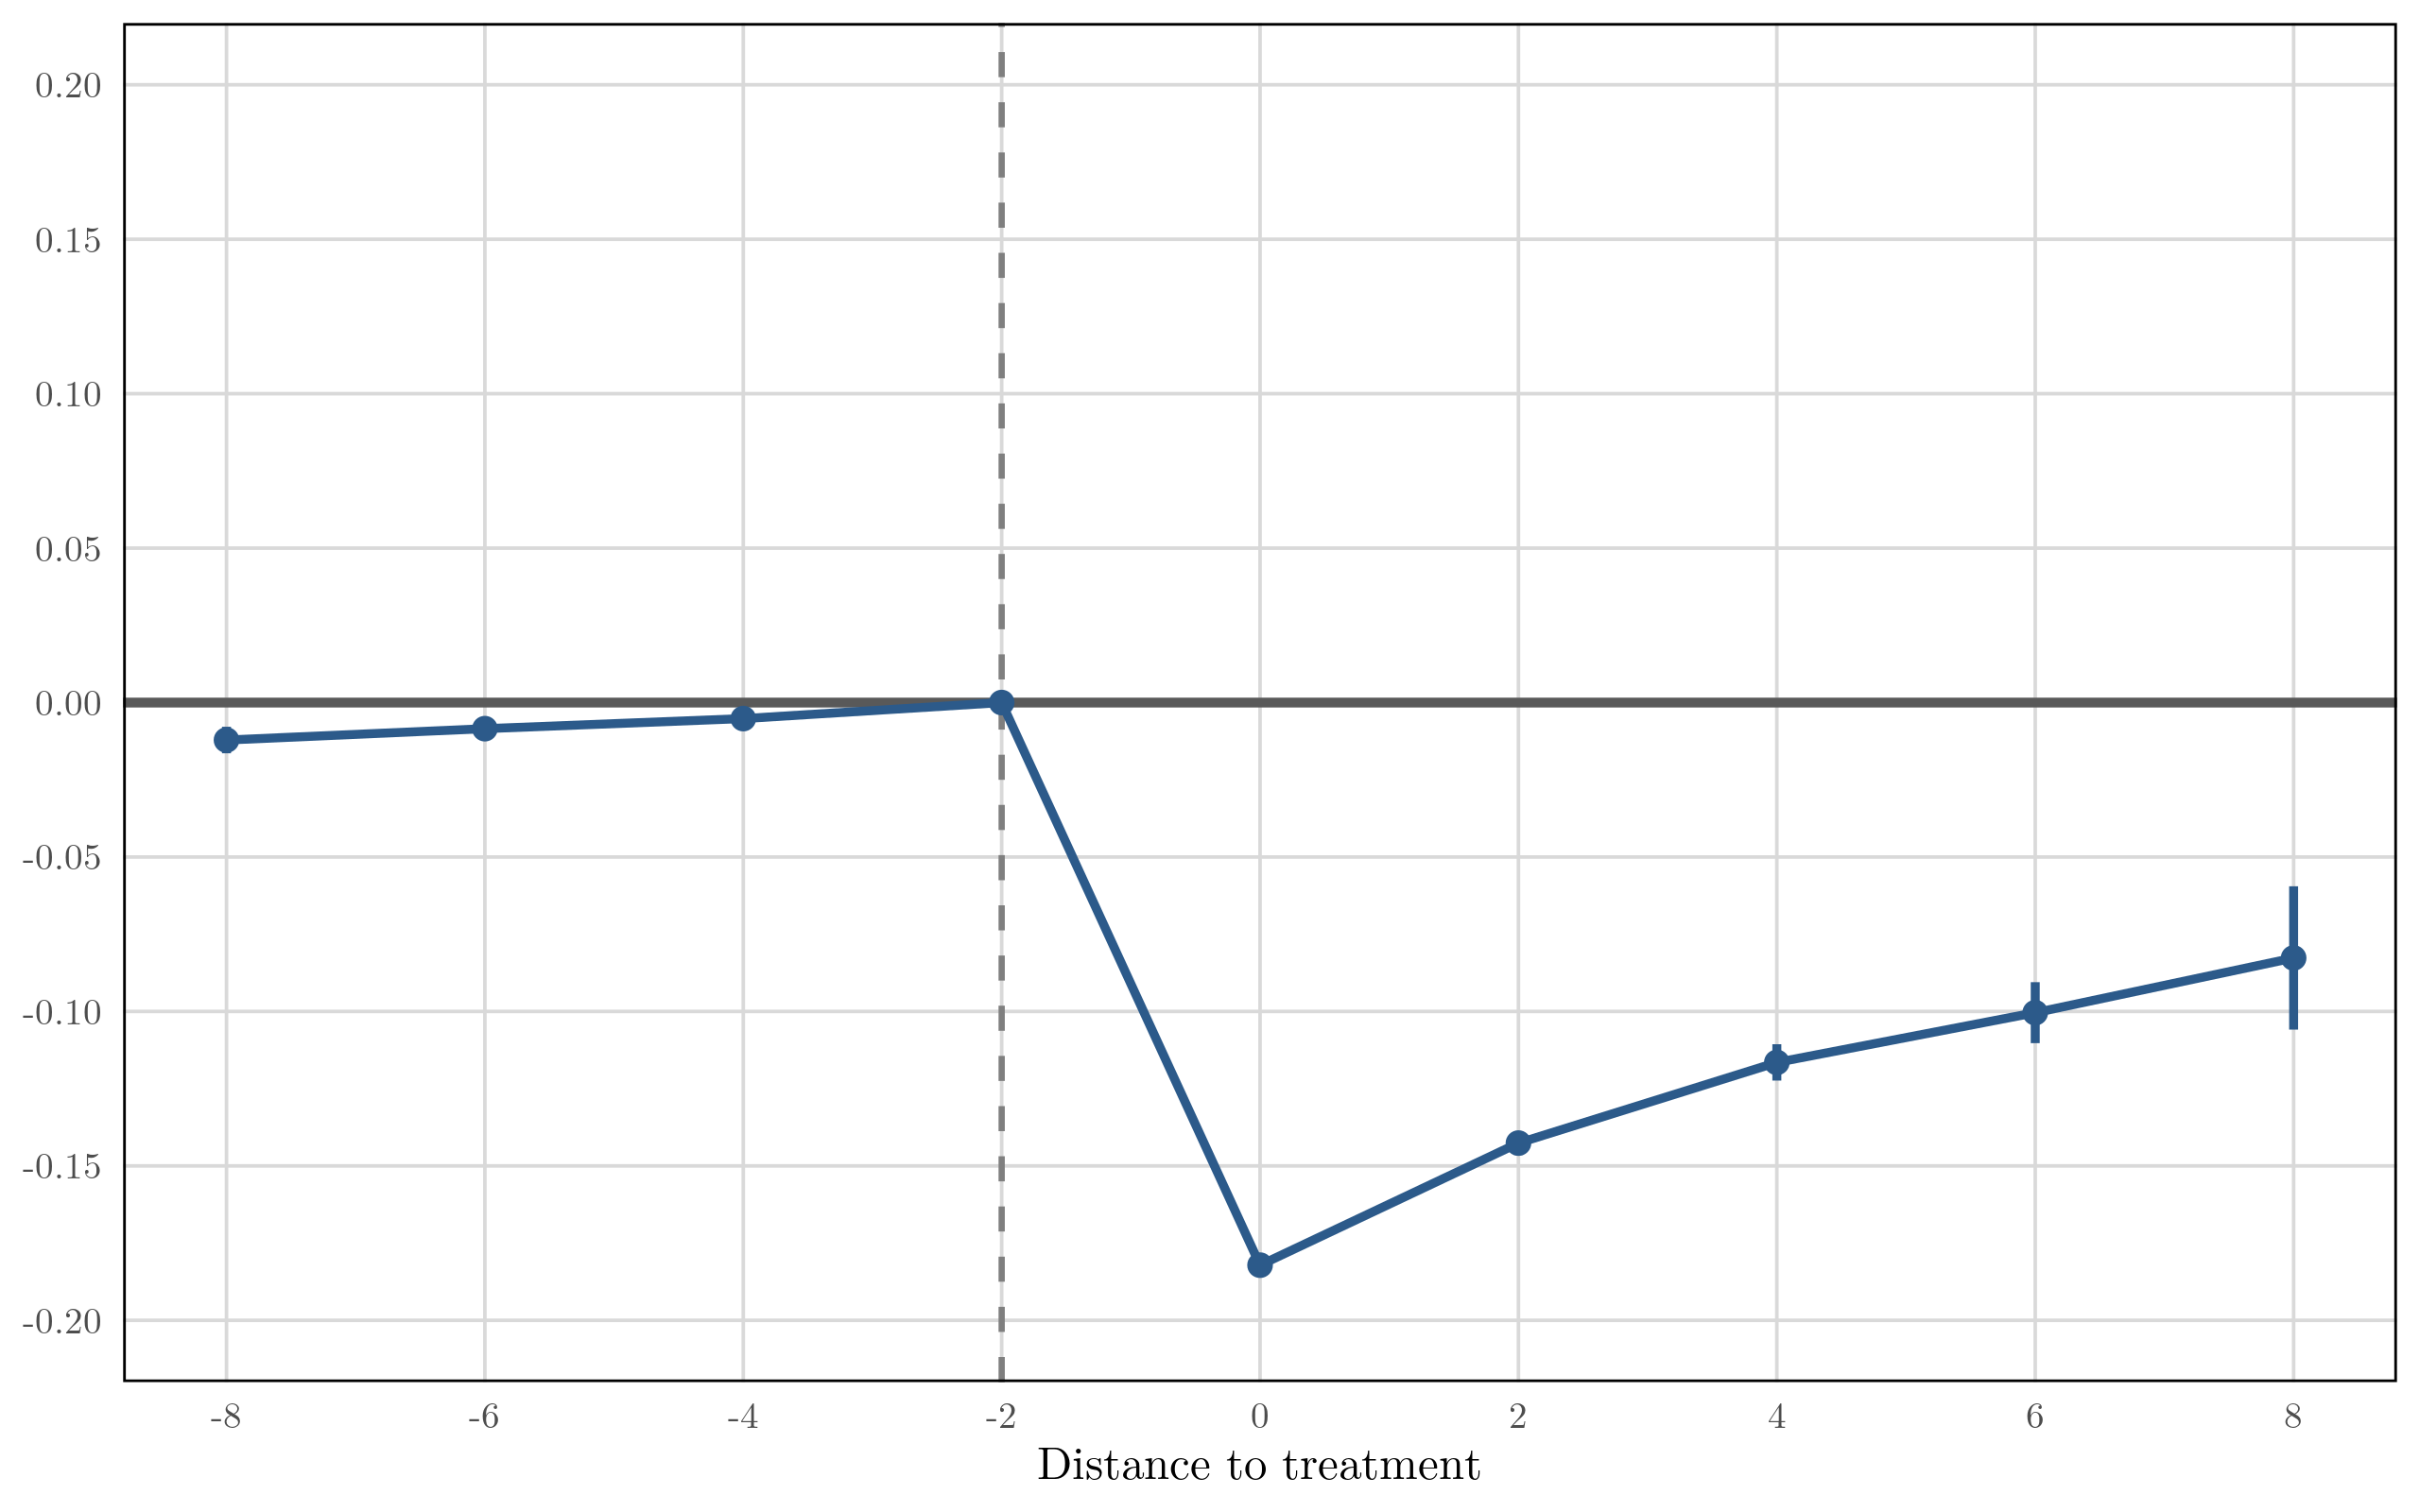
\includegraphics[width=\textwidth]{../resources/regressions/decomposition/low_ed_over_2006/strict_bvr/callaway_santanna/event_study_plot.png}
        \caption{Low education over 2006 total}
        \label{fig:appendix-decomp-event-low-ed}
    \end{subfigure}
    \par\medskip
    \begin{subfigure}[b]{0.49\textwidth}
        \centering
        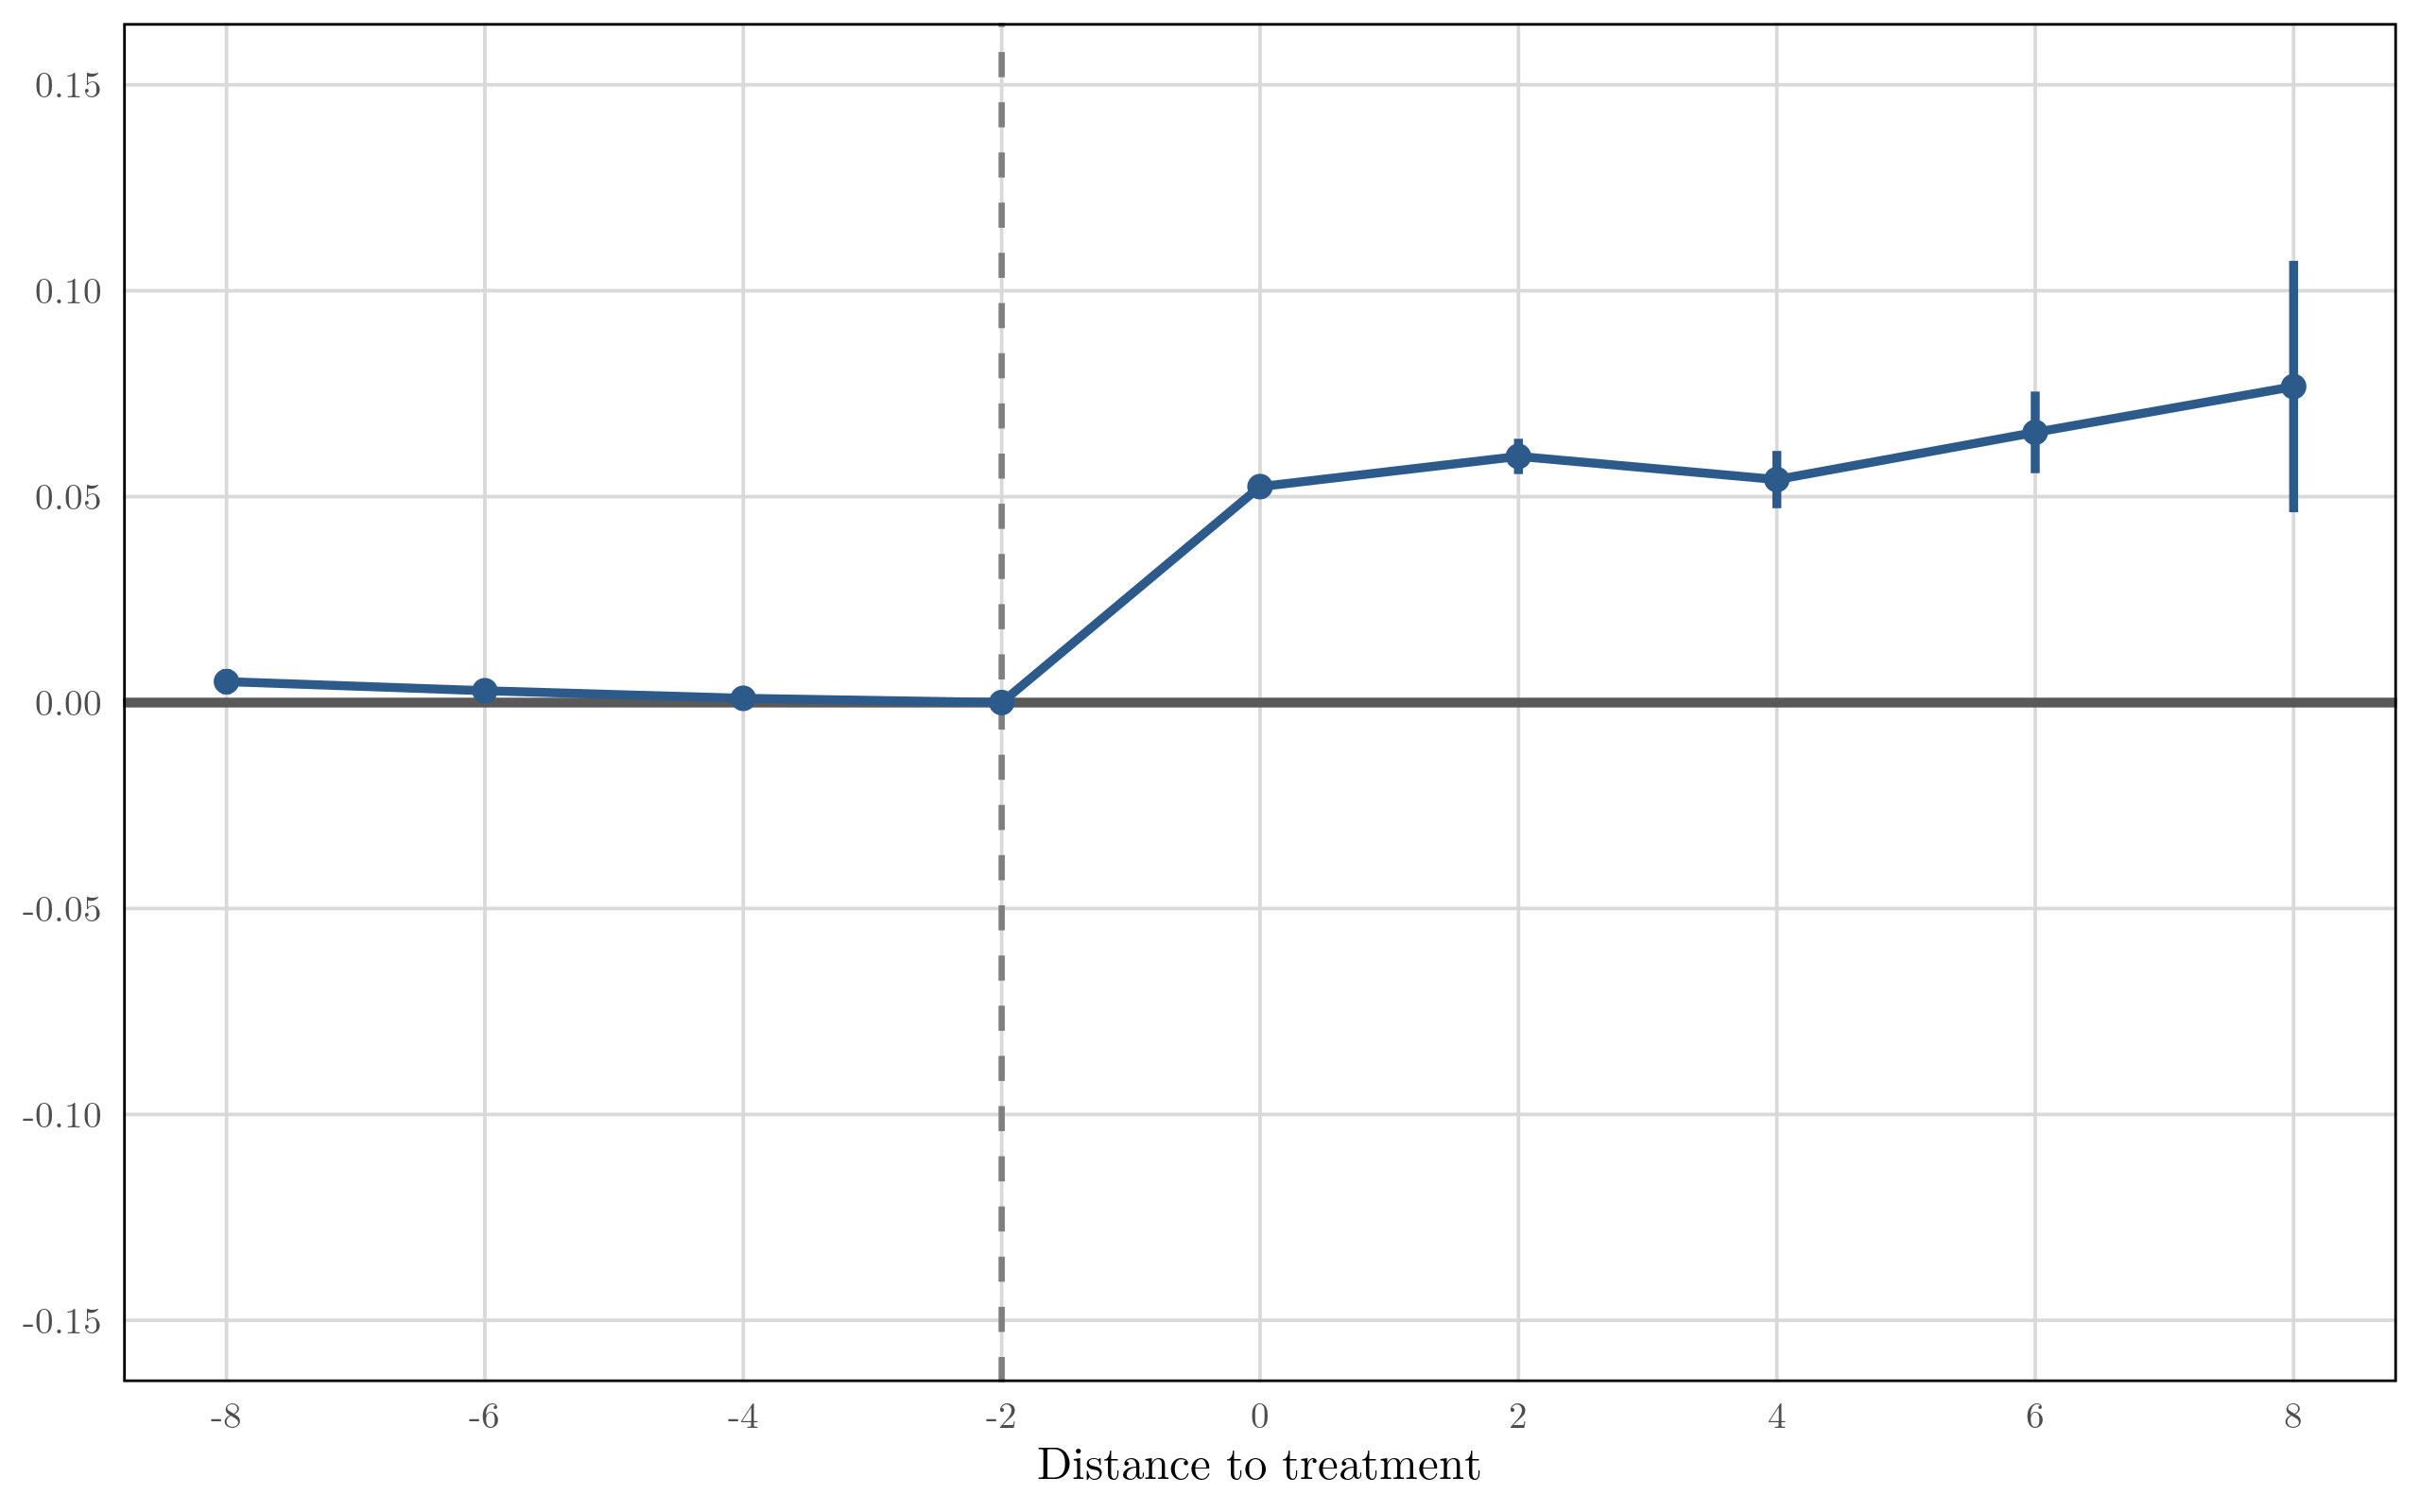
\includegraphics[width=\textwidth]{../resources/regressions/decomposition/high_ed_over_2006/strict_bvr/callaway_santanna/event_study_plot.png}
        \caption{High education over 2006 total}
        \label{fig:appendix-decomp-event-high-ed}
    \end{subfigure}
    \hfill
    \begin{subfigure}[b]{0.49\textwidth}
        \centering
        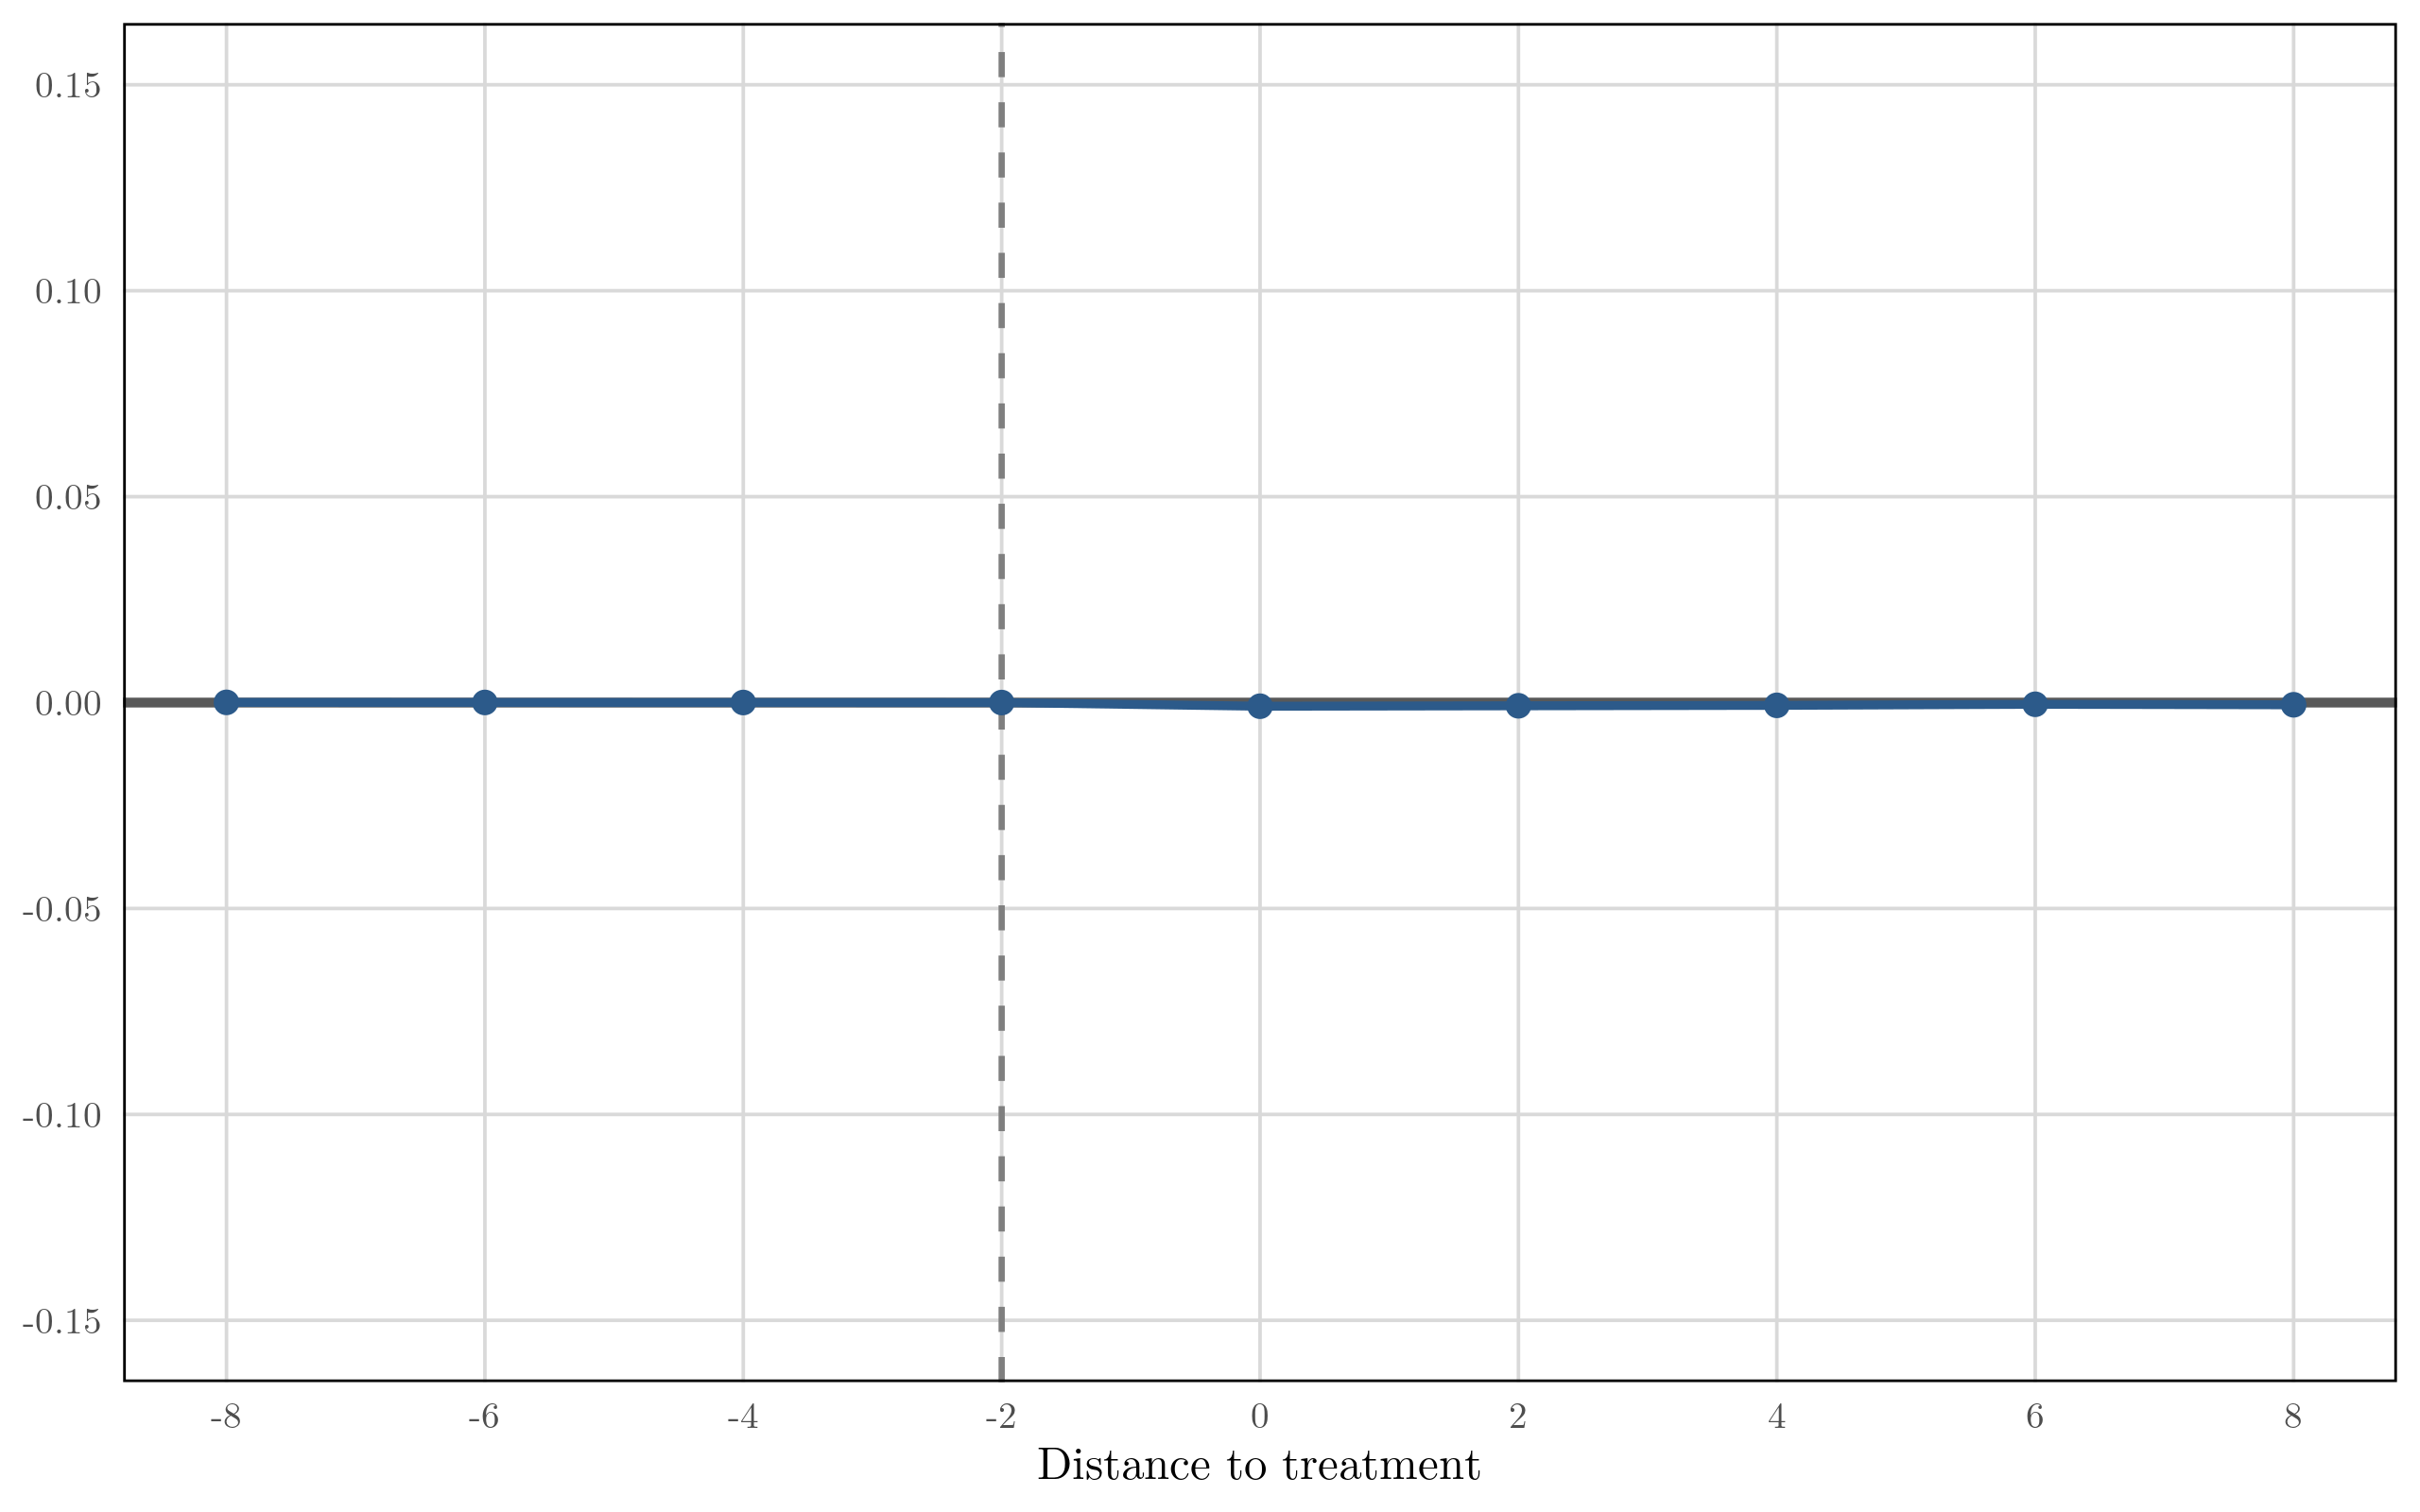
\includegraphics[width=\textwidth]{../resources/regressions/decomposition/unknown_ed_over_2006/strict_bvr/callaway_santanna/event_study_plot.png}
        \caption{Unknown education over 2006 total}
        \label{fig:appendix-decomp-event-unknown-ed}
    \end{subfigure}
    \vspace{0.75em}
    \begin{minipage}{\textwidth}
        {\footnotesize \textbf{Note:} Each panel plots BJS imputation event-study estimates \citep{Borusyak2024RevisitiEventStudy} using strict BVR municipalities as the treated sample and never-treated municipalities as the control group. Panel (a) uses total registered voters divided by the municipality's 2006 registered voters. Panels (b)--(d) use the corresponding low-education, high-education, and unknown-education counts divided by the municipality's 2006 total registered voters. Event time $-2$ is the reference period and is shown at zero. Error bars report 95\% confidence intervals with standard errors clustered by municipality. The component outcomes add to the total-electorate outcome by construction in the underlying data. \par}
    \end{minipage}
\end{figure}

